\chapter{System Design}
Provide a detailed explanation of the overall system architecture \cite{lin1991divergence}, i.e. the HOW of the project.
Use UML, system architecture diagrams, screenshots, code snippets and algorithms to illustrate your design.

\subsection*{Legacy Architecture}

The entire system architecture, as designed in the previous projects, is visualized in \autoref{fig:systemArchitecture}. This system consists of three modules that interact with both an external API and user devices. These modules are detailed as follows:

\begin{itemize}
\item{Test Application}\\
A Unity-designed desktop application on a Windows Platform where users can play tests for different game scenarios.
\item {Node Js Web Application}\\
An Express Node JS Web application deployed on Amazon EC2 Virtual machine, serving as a callback endpoint for OAuth 2.0 Authentication for the Polar Flow API. 
\item {Firestore Data Storage}\\
Permanent storage medium for user's test and Biometric data.
\end{itemize}
User Devices:
\begin{itemize}
\item{Smart Watch}
\item {Smart Phone}
\end{itemize}

\begin{figure}[h]
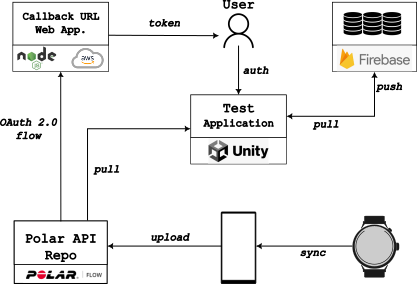
\includegraphics{images/architecture.png}
\caption{System Architecture}
\label{fig:systemArchitecture}
\centering
\end{figure}

The actions in the Figure \autoref{fig:systemArchitecture} can be summarized as follows:
\begin{itemize}
\item{sync}: passing of biometric data to a smartphone from a Polar watch.
\item {upload}: uploading of biometric data to Polar API repository.
\item {OAuth 2.0 flow}: Multi step OAuth 2.0 authentication protocol. 
\item {token}: getting verification token from the Callback URL by the user.
\item {pull (Polar API - Test Application)}: retrieving biometric data from Polar API by the Test Application.
\item {auth}: The user supplies a token to the Test Application as a final step of authentication. 
\item {pull (Firebase - Test Application)}: retrieving user test/biometric data for rendering by Test Application.
\item {push}: saving user's test/biometric data to a Datastore.
\end{itemize}

\subsection*{Proposed Architecture}
The final system architecture will include new modules to facilitate data analytics using AI models. The new system calls for a relational database replica of the Firebase storage to ensure data consistency, predictability and structures suitable for relevant statistical analysis. A.I models as a mini-service that performs operations with supplied data and returns the result of the analysis. A Web Application that functions as a Controller that interfaces the data and A.I modules, Executive Dashboard that renders user data and results from the A.I models and any other information about the system.\\
\autoref{fig:proposed_web_architecture} shows the proposed architectural layout for the System.\\


\begin{figure}[h]
    \centering
    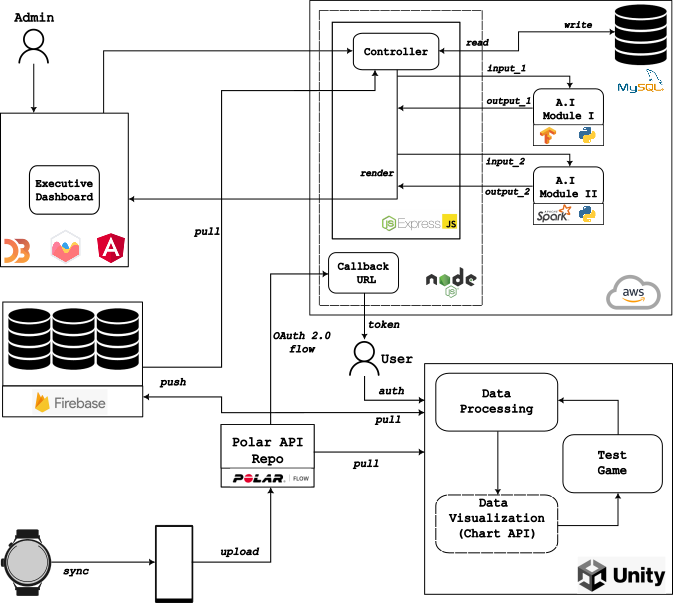
\includegraphics[scale=1]{images/new-arch.png}
    \caption{Web Application Architecture}
    \label{fig:proposed_web_architecture}
\end{figure}


Additional modules have been added to the web application namely back end `Controller' \& front end `Executive Dashboard', and a 'Relational Database'. The functions of these modules are explained below:

\begin{itemize}
\item {Controller}: This module is responsible for coordinating data fetch from the Relational Database and making sure that the Relational Database is always in sync with the Firebase Datastore. It is also responsible for filtering and structuring data being fed into the A.I. Modules and when necessary using the output for an A.I module as input for another A.I module. 
\item{Executive Dashboard}: This module provides a Graphical User Interface that displays the working dataset, and offers interfaces to filter, tune and if needed bias the data being sent to the A.I Modules for analysis. This module will developed using the Angular Framework with integration of D3.js or Chart.js for displaying relevant charts. The choice for Angular Framework over other solutions namely ReactJS and Vue is because of the more structured Angular Framework which is more suited for collaborative work.
\item{A.I Modules}: These modules are responsible for running analysis on data. The modules accept input from the `Controller' and output a comprehensive summary of the results of the analysis done to the `Executive Dashboard' module. For this purpose, TensorFlow and Apache Spark were chosen for the following reasons:
\end{itemize}

\begin{itemize}
    \item {Capabilities}: Apache Spark is capable of performing linear and logical regression\cite{apache_spark} which are common tools used for this class of problem. TensorFlow also has the same capabilities and can perform regression neural network models\cite{tensor_flow}.
    \item {Accessibility}: Both tools are open-source and available to the general public\cite{open_source}.
    \item{Python API interface}: Both tools provide a Python API. This eases deployment as Python is platform-independent and relatively easy setup in a Ubuntu Virtual machine.
    \item{Large Community}: Both have a large community of contributors. Documentation and tutorials are vastly available on the internet.
    \item{Relational Database}: Data for the analysis will be sourced directly from this Database which is a structured replica of the FireStore Database as obtained from the Legacy System. The rationale for this Module is to provide a flexible means of retrieving data in various forms and shapes as may be needed for analysis and also overcome the high complexities involved in FireStore for compound queries.
    \item{Chart API}:
    Is responsible for displaying test results and biometric data to the users. This already developed module will be integrated into the 'Test Application' and undergo some modification to be able to display custom data as requirements change. 
    
\end{itemize}